\documentclass[11pt,a4paper]{article}
\usepackage[margin=2.2cm]{geometry}
\usepackage[expansion=false]{microtype}
\usepackage{graphicx}
\usepackage{booktabs}
\usepackage{tabularx}
\usepackage{xcolor}
\usepackage{listings}
\usepackage{enumitem}
\usepackage[hidelinks]{hyperref}

\definecolor{codebg}{HTML}{F5F7FA}
\definecolor{accent}{HTML}{1D4ED8}
\lstset{basicstyle=\ttfamily\small, backgroundcolor=\color{codebg}, frame=single, rulecolor=\color{gray!40},
        columns=fullflexible, keepspaces=true, showstringspaces=false, breaklines=true, xleftmargin=4pt, xrightmargin=4pt,
        keywordstyle=\color{accent}\bfseries, commentstyle=\color{gray}\itshape}
\setlist{itemsep=2pt, topsep=4pt}
\graphicspath{{../results/}}

\title{\textbf{ESP32-S3 GDMA Bus-Contention Profiler}\\[4pt]
       \large Design, measurements and findings}
\author{Parth Sinha}
\date{October 2026}

\begin{document}
\maketitle

\begin{abstract}
\noindent This report describes a profiler that measures how General DMA (GDMA) traffic on the
ESP32-S3 interferes with 128-bit PIE SIMD workloads running on the other CPU core. Core~1 runs four
vector kernels (read, write, copy and stride) over internal SRAM and external octal PSRAM, while
Core~0 keeps the GDMA engine saturated with memory-to-memory transfers. A host script requests a
27-cell measurement matrix over a native USB vendor interface and produces a CSV file and a plot.
When GDMA writes into PSRAM, every CPU workload in PSRAM slows down by 41--69\,\%, and the DMA
throughput itself falls from 36.4\,MB/s to 12--18\,MB/s. SRAM workloads lose less than 8\,\% in every
configuration. The same firmware streams GDMA-filled ping-pong buffers to the host at 1.18\,MB/s,
which is 97\,\% of the USB full-speed bulk limit, with no data loss under any Core~1 load.
\end{abstract}

\tableofcontents
\newpage

%--------------------------------------------------------------------
\section{Goals}
The project set out to answer three questions:
\begin{enumerate}
  \item How much does concurrent GDMA traffic slow a SIMD workload on the other core, and how does
        this depend on where the data lives (SRAM or PSRAM) and on the access pattern?
  \item How much does the CPU workload, in turn, slow the DMA engine?
  \item Can a GDMA-fed producer stream data to a PC over USB without loss while the other core is
        under heavy memory load?
\end{enumerate}
The work was organised in five phases (0--4), summarised in Table~\ref{tab:phases}.

\begin{table}[h]
\centering
\begin{tabularx}{\linewidth}{@{}lX@{}}
\toprule
Phase & Outcome \\
\midrule
0 Baseline & GDMA M2M pump on Core~0, PIE read kernel on Core~1, first contention table \\
1 USB bulk & TinyUSB vendor class with bulk IN/OUT; per-packet ZLP problem fixed \\
2 Ping-pong & Two GDMA-filled 4\,KB buffers streamed over USB; backpressure and paced modes \\
3 SIMD engine & Read, write, copy and stride kernels; full kernel $\times$ memory $\times$ GDMA matrix \\
4 Analytics & Profiling on request over USB; host computes rates, writes CSV and PNG \\
\bottomrule
\end{tabularx}
\caption{Project phases.}
\label{tab:phases}
\end{table}

%--------------------------------------------------------------------
\section{Platform}
\subsection{Hardware}
\begin{itemize}
  \item ESP32-S3 N16R8 module: dual-core Xtensa LX7 at 240\,MHz, 16\,MB flash, 8\,MB octal PSRAM at 80\,MHz.
  \item 32\,KB data cache with 32\,B lines in front of PSRAM.
  \item Two USB connectors: a CH343 USB--UART bridge (\texttt{/dev/ttyACM1}) used for flashing and
        the console, and the native USB-OTG port, which enumerates as vendor device \texttt{303a:4020}.
\end{itemize}

\subsection{Software}
ESP-IDF v5.3, FreeRTOS with a 100\,Hz tick, and the \texttt{espressif/esp\_tinyusb} component
($\geq$\,1.4). Host scripts are written in Python and run with \texttt{uv} using \texttt{pyusb}
and \texttt{matplotlib}.

\subsection{Hardware limits that shaped the design}
Three constraints of the chip changed the original plan:
\begin{itemize}
  \item \textbf{GDMA cannot feed USB-OTG.} The USB controller has its own DMA engine; GDMA serves
        SPI2/3, UHCI, I2S, LCD/CAM, AES, SHA, ADC, RMT and memory-to-memory transfers. The stream
        therefore uses GDMA to fill a buffer and the CPU to hand it to TinyUSB.
  \item \textbf{PIE SIMD is integer only.} There are no 128-bit floating-point vectors, so the
        kernels are pure 128-bit load/store streams.
  \item \textbf{USB is full speed only} (12\,Mbit/s). The practical bulk ceiling is 1.216\,MB/s.
\end{itemize}

%--------------------------------------------------------------------
\section{System architecture}
Work is split between the two cores so that the DMA load generator and the measured workload never
share a CPU (Table~\ref{tab:tasks}).

\begin{table}[h]
\centering
\begin{tabularx}{\linewidth}{@{}lllX@{}}
\toprule
Task & Core & Priority & Role \\
\midrule
\texttt{dma\_pump}   & 0 & 10 & Keeps two GDMA M2M transfers queued while a DMA mode is active \\
\texttt{usb\_stream} & 0 & 6  & Moves ready ping-pong buffers into TinyUSB \\
TinyUSB task         & 0 & 5  & USB device stack (pinned to Core~0 in \texttt{sdkconfig.defaults}) \\
\texttt{profiler}    & 1 & 5  & Runs the profile matrix, or a stream load kernel \\
\bottomrule
\end{tabularx}
\caption{FreeRTOS tasks.}
\label{tab:tasks}
\end{table}

\noindent The host talks to the board over one bulk OUT and one bulk IN endpoint. It sends either a
4-byte \texttt{PROF} command, which starts a profile, or a 12-byte stream request
(Section~\ref{sec:protocol}).

%--------------------------------------------------------------------
\section{Firmware design}
\subsection{GDMA load generator}
\texttt{dma\_pump} uses the ESP-IDF async memcpy driver on a GDMA AHB channel. Each transfer moves
32\,KB from an internal SRAM source buffer to either a second SRAM buffer or a PSRAM buffer. A counting
semaphore with two slots keeps two transfers in flight, so the channel never idles between
transfers; this raised SRAM-to-SRAM throughput from 59 to 61.6\,MB/s. The completion ISR adds the
transfer length to a byte counter, from which the host later derives the DMA rate.

\subsection{PIE SIMD kernels}
All four kernels are written in inline assembly with the Xtensa zero-overhead loop
(\texttt{loopnez}) and the PIE post-increment instructions \texttt{ee.vld.128.ip} and
\texttt{ee.vst.128.ip}. Each kernel sweeps the same address span, so cycles per KB are comparable.

\begin{table}[h]
\centering
\begin{tabularx}{\linewidth}{@{}lX@{}}
\toprule
Kernel & Access pattern \\
\midrule
\texttt{k\_read}   & Four 16\,B loads per loop iteration, contiguous \\
\texttt{k\_write}  & Four 16\,B stores per loop iteration, contiguous \\
\texttt{k\_copy}   & Copies the first half of the buffer to the second half \\
\texttt{k\_stride} & One 16\,B load per 32\,B cache line, so on PSRAM every load is a line miss \\
\bottomrule
\end{tabularx}
\caption{PIE kernels.}
\end{table}

\begin{lstlisting}[language=C, caption={Read kernel.}]
asm volatile(
    "loopnez %1, 1f\n"
    "ee.vld.128.ip q0, %0, 16\n"
    "ee.vld.128.ip q1, %0, 16\n"
    "ee.vld.128.ip q2, %0, 16\n"
    "ee.vld.128.ip q3, %0, 16\n"
    "1:\n"
    : "+r"(buf) : "r"(len / 64) : "memory");
\end{lstlisting}

\noindent Workload buffers are 64\,KB in SRAM and 256\,KB in PSRAM. The PSRAM buffer is eight times
larger than the data cache, so every pass misses.

\subsection{Measurement method}
For each cell, \texttt{run\_cell} sets the GDMA mode, waits 20\,ms for the pump to reach steady
state, then runs the kernel repeatedly. It runs at least 50 times and for at least 100\,ms, so many
DMA completions fall inside the window. The CPU cycle counter gives the best and summed cycles per
run; the DMA byte counter gives the bytes moved in the same window. The device sends only raw
counters; the host derives every rate.

The matrix has 27 cells: four kernels on SRAM, the read kernel on the GDMA source buffer
(SRAM$^*$), and four kernels on PSRAM, each under three GDMA modes (idle, SRAM$\to$SRAM,
SRAM$\to$PSRAM).

\subsection{Ping-pong stream}
Two 4\,KB DMA-capable SRAM buffers move through the states \textsc{free} $\to$ \textsc{filling}
$\to$ \textsc{ready}. \texttt{produce()} claims the next free buffer, writes an 8-byte header
\{\texttt{seq}, \texttt{overruns}\}, and starts a GDMA copy of a fixed incrementing-word pattern into
the rest of the block. The completion ISR marks the buffer ready and notifies \texttt{usb\_stream},
which passes it to \texttt{tud\_vendor\_write} and frees it.

\begin{itemize}
  \item \textbf{Backpressure mode} (interval 0): the next block is produced as soon as a buffer is
        free. Nothing is lost and throughput is limited by USB.
  \item \textbf{Paced mode} (interval $>0$): an \texttt{esp\_timer} produces one block per tick, as a
        sampling peripheral would. A tick that finds its buffer still owned by USB counts an overrun
        and advances \texttt{seq}, so the host sees exactly one sequence gap per dropped block.
\end{itemize}

\subsection{USB configuration}
TinyUSB's buffered vendor mode drains a 64\,B FIFO and appends a zero-length packet after every
packet. The top-level \texttt{CMakeLists.txt} switches to unbuffered mode with 4\,KB IN transfers
(\texttt{CFG\_TUD\_VENDOR\_TXRX\_BUFFERED=0}, \texttt{CFG\_TUD\_VENDOR\_TX\_EPSIZE=4096}), so each block
is one transfer.

%--------------------------------------------------------------------
\section{Wire protocol}
\label{sec:protocol}
\begin{table}[h]
\centering
\begin{tabularx}{\linewidth}{@{}llX@{}}
\toprule
Direction & Message & Layout (little endian) \\
\midrule
OUT & Stream request & \texttt{u32 blocks, u32 interval\_us, u32 load}; \texttt{load} = kernel $|$ 0x10 for PSRAM \\
IN  & Stream block   & \texttt{u32 seq, u32 overruns}, then 4088\,B pattern \\
OUT & Profile request& ASCII \texttt{PROF} (4 bytes) \\
IN  & Profile reply  & One 4096\,B block: \texttt{'PROF', u32 count, u32 cpu\_mhz, u32 32}, then \texttt{count} cells \\
\bottomrule
\end{tabularx}
\caption{USB messages.}
\end{table}

\begin{lstlisting}[language=C, caption={Profile cell (32 bytes).}]
typedef struct {
    uint8_t  mem, kernel, gdma, pad;
    uint32_t len, runs, best, elapsed, dma_bytes;  // cycles, except len/dma_bytes
    uint64_t sum;                                  // cycles over all runs
} cell_t;
\end{lstlisting}

%--------------------------------------------------------------------
\section{Host tools}
\begin{itemize}
  \item \texttt{host/usbdev.py} opens \texttt{303a:4020} and drains data left over from an interrupted run.
  \item \texttt{host/stream.py [blocks] [interval\_us] [load]} measures throughput, checks every block
        against the pattern, and verifies that sequence gaps equal the device's overrun count.
  \item \texttt{host/profile.py [prefix] [--replot]} requests the matrix, prints it with slowdown
        relative to the idle bus, and writes \texttt{<prefix>.csv} and \texttt{<prefix>.png}.
\end{itemize}

%--------------------------------------------------------------------
\section{Results}
\subsection{USB streaming}
\begin{table}[h]
\centering
\begin{tabular}{@{}lrrr@{}}
\toprule
Mode & Offered (MB/s) & Delivered (MB/s) & Dropped \\
\midrule
Backpressure & -- & 1.182 & 0 \\
Paced, 5000\,$\mu$s & 0.819 & 0.818 & 0 \\
Paced, 4000\,$\mu$s & 1.024 & 1.022 & 0 \\
Paced, 3000\,$\mu$s & 1.365 & 1.180 & 76 of 576 (13.2\,\%) \\
\bottomrule
\end{tabular}
\caption{Stream throughput. In the overloaded case, sequence gaps matched the device overrun count exactly.}
\end{table}

\noindent Running any of the eight kernel/memory loads on Core~1 during the stream changed neither
the stream throughput (1.18\,MB/s in backpressure mode) nor the drop count (zero at 3500\,$\mu$s),
and the Core~1 rates were unchanged as well. The stream uses about 2\,\% of SRAM bandwidth, and USB
full speed is the bottleneck, so contention cannot appear on this path.

\subsection{Contention matrix}
Table~\ref{tab:matrix} gives average cycles per KB for each workload, with the change relative to
an idle bus. Figure~\ref{fig:profile} shows the same data.

\begin{table}[h]
\centering
\small
\begin{tabular}{@{}llr r rr rr@{}}
\toprule
 & & CPU idle & idle & \multicolumn{2}{c}{GDMA SRAM$\to$SRAM} & \multicolumn{2}{c}{GDMA SRAM$\to$PSRAM} \\
\cmidrule(lr){5-6}\cmidrule(lr){7-8}
Memory & Kernel & MB/s & c/KB & c/KB & \% & c/KB & \% \\
\midrule
SRAM & read & 3821.1 & 64.3 & 66.6 & +3.6 & 64.4 & +0.1 \\
SRAM & write & 3821.4 & 64.3 & 66.6 & +3.6 & 64.4 & +0.1 \\
SRAM & copy & 3818.3 & 64.4 & 68.9 & +7.0 & 64.7 & +0.5 \\
SRAM & stride & 7609.1 & 32.3 & 33.5 & +3.6 & 32.3 & +0.1 \\
SRAM$^*$ & read & 3804.8 & 64.6 & 69.5 & +7.6 & 67.1 & +3.9 \\
\midrule
PSRAM & read & 62.4 & 3939.7 & 3939.6 & 0.0 & 6659.5 & \textbf{+69.0} \\
PSRAM & write & 35.1 & 7004.9 & 7012.5 & +0.1 & 9853.3 & \textbf{+40.7} \\
PSRAM & copy & 44.5 & 5527.5 & 5523.6 & $-$0.1 & 8260.3 & \textbf{+49.4} \\
PSRAM & stride & 62.3 & 3943.1 & 3939.3 & $-$0.1 & 6657.9 & \textbf{+68.8} \\
\bottomrule
\end{tabular}
\caption{Average CPU cycles per KB at 240\,MHz. SRAM$^*$ means the CPU reads the GDMA source buffer.
CPU MB/s is address span per second, so stride, which touches half the bytes, shows twice the read rate.}
\label{tab:matrix}
\end{table}

\begin{table}[h]
\centering
\begin{tabular}{@{}lrr@{}}
\toprule
CPU workload & GDMA SRAM$\to$SRAM (MB/s) & GDMA SRAM$\to$PSRAM (MB/s) \\
\midrule
Any SRAM workload & 61.6 & 36.4 \\
PSRAM read   & 61.8 & 18.1 \\
PSRAM write  & 61.7 & 12.3 \\
PSRAM copy   & 61.6 & 14.7 \\
PSRAM stride & 61.6 & 18.0 \\
\bottomrule
\end{tabular}
\caption{GDMA throughput while the CPU runs each workload.}
\label{tab:gdma}
\end{table}

\begin{figure}[!htb]
\centering
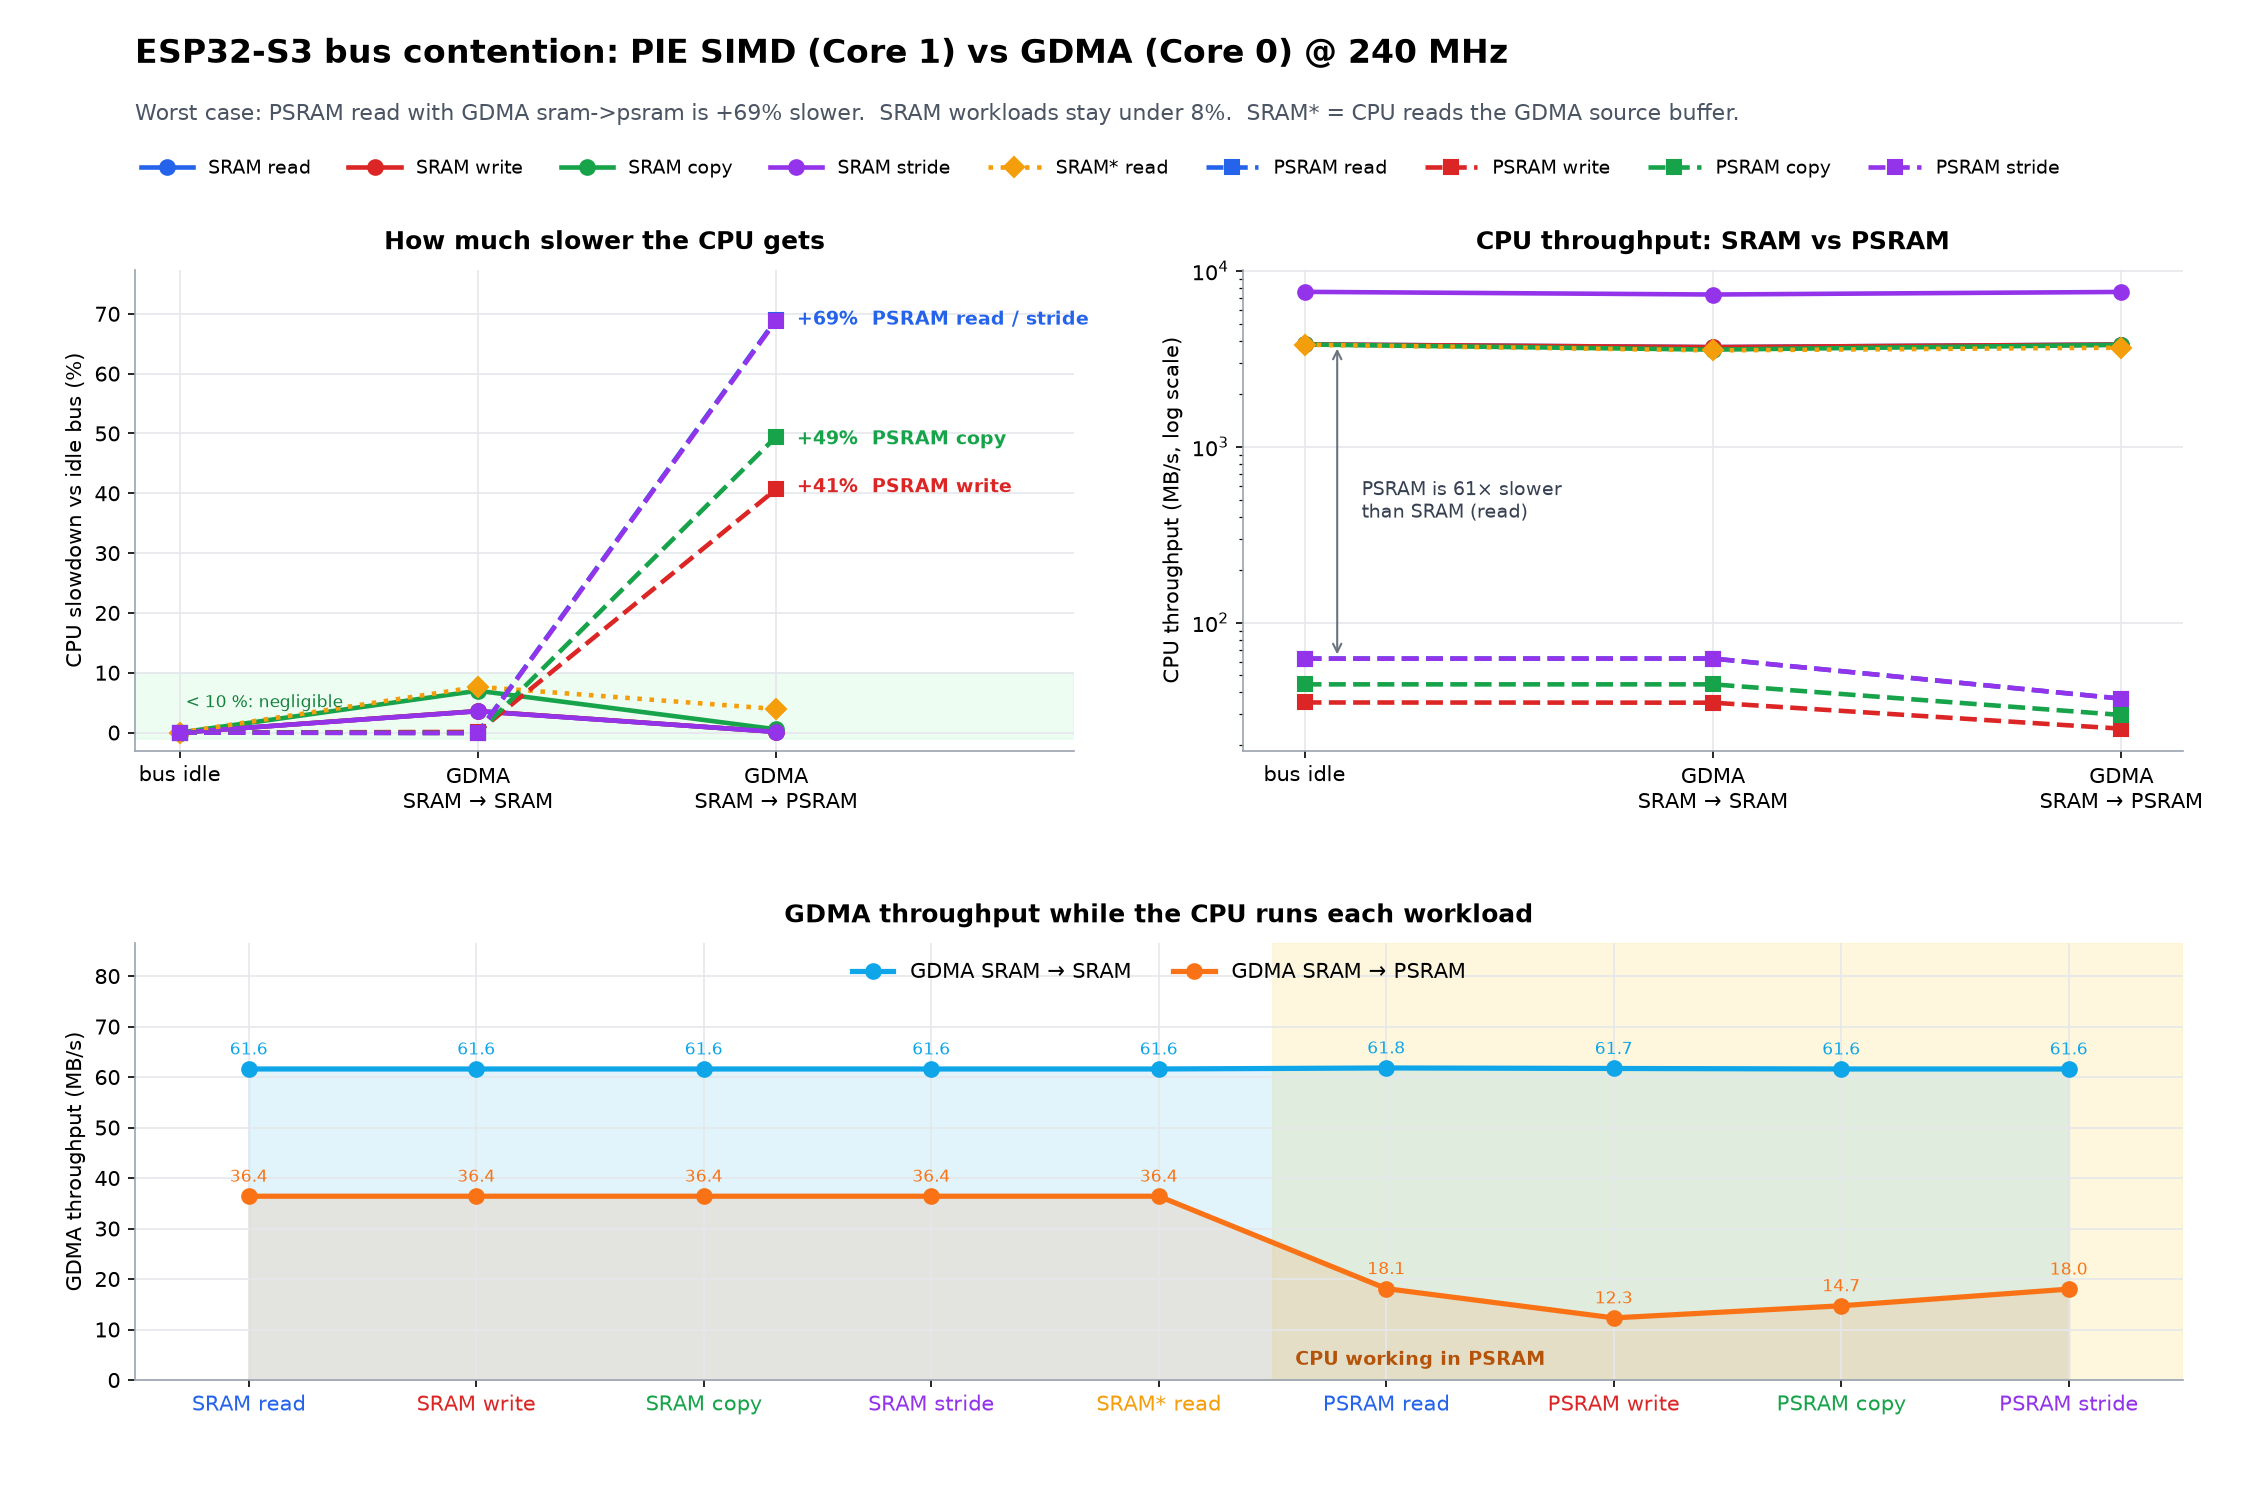
\includegraphics[width=\linewidth]{profile.png}
\caption{Contention profile. Top left: CPU slowdown relative to an idle bus. Top right: CPU
throughput on a log scale. Bottom: GDMA throughput while the CPU runs each workload.}
\label{fig:profile}
\end{figure}

\subsection{Discussion}
\begin{itemize}
  \item \textbf{SRAM costs one cycle per 16 bytes} regardless of access pattern. GDMA traffic into the
        same SRAM adds 2--7\,\%, and up to 7.6\,\% when the CPU reads the very buffer GDMA is reading.
        GDMA into PSRAM barely touches SRAM workloads.
  \item \textbf{PSRAM is bound by cache-line fills.} The stride kernel, which loads only one 16\,B
        vector per line, costs the same as reading every byte. Writes cost about 1.8$\times$ reads
        because each line is both filled and later written back. With an idle bus, reading SRAM is
        about 61$\times$ faster than reading PSRAM.
  \item \textbf{GDMA into PSRAM is the dominant source of contention.} CPU workloads in PSRAM slow by
        41--69\,\%, and the effect is mutual: GDMA throughput into PSRAM falls from 36.4\,MB/s to
        12--18\,MB/s, with the write kernel, which generates the most PSRAM traffic, hurting it most.
  \item \textbf{GDMA SRAM$\to$SRAM does not affect PSRAM workloads}, and PSRAM workloads do not slow it.
\end{itemize}
\noindent The practical conclusion is that data placement matters far more than DMA scheduling.
Keeping either the CPU's working set or the DMA destination in internal SRAM removes nearly all of
the interference.

%--------------------------------------------------------------------
\section{Problems found and fixed}
\begin{description}[style=nextline]
  \item[Zero-length packet after every USB packet.] TinyUSB's buffered vendor mode sent a ZLP after
        each 64\,B packet. Switching to unbuffered mode with 4\,KB transfers fixed it.
  \item[10\,ms per block in backpressure mode (0.41\,MB/s).] The streaming task busy-polled at idle
        priority, so the idle task on Core~0 executed \texttt{waiti} and slept until the next 10\,ms
        tick. The task now blocks on notifications from the GDMA ISR and from
        \texttt{tud\_vendor\_tx\_cb}, and runs at priority 6. Throughput rose to 1.18\,MB/s.
  \item[Stream fell to 0.41\,MB/s under any Core~1 load.] The TinyUSB task defaulted to Core~1 at
        priority 5 and shared time slices with the busy workload. Pinning it to Core~0
        (\texttt{CONFIG\_TINYUSB\_TASK\_AFFINITY\_CPU0}) fixed it.
  \item[\texttt{esp\_timer\_stop} inside a critical section.] Moved outside the spinlock.
\end{description}

%--------------------------------------------------------------------
\section{Reproducing the results}
One-time setup: add the user to \texttt{dialout} and install a udev rule for \texttt{303a:4020}
(see \texttt{README.md}). Then, from the project folder:
\begin{lstlisting}[language=bash]
. ~/esp/esp-idf/export.sh
idf.py -p /dev/ttyACM1 flash monitor          # Ctrl+] exits

# in a second terminal
uv run --with pyusb host/stream.py 1000                     # max throughput
uv run --with pyusb host/stream.py 500 3000                 # paced, overruns
uv run --with pyusb host/stream.py 500 3500 psram:write     # stream under load
uv run --with pyusb --with matplotlib host/profile.py results/profile
\end{lstlisting}
Each stream test prints \texttt{data OK} when it passes. To rebuild this report, run
\texttt{pdflatex report.tex} twice in \texttt{docs/}.

%--------------------------------------------------------------------
\section{Limitations and future work}
\begin{itemize}
  \item The stream producer is a memory-to-memory copy driven by a timer. A real peripheral source
        (I2S RX or continuous ADC) would exercise a true peripheral DMA path.
  \item Placing the ping-pong buffers in PSRAM would make the stream compete with PSRAM workloads.
  \item GDMA burst size, transfer size and PSRAM clock (80 versus 120\,MHz) were not swept.
  \item The matrix has no ``USB active'' dimension, because the stream showed no measurable effect.
\end{itemize}

\end{document}
